\section{Ziel}
In diesem Versuch sollen die Grundlagen der Ultraschalltechnik mitsamt den wichtigen Begriffen und den pyhsikalischen Eigenschaften kennengelernt werden.
\section{Theorie}
\label{sec:Theorie}

Der Ultraschallbereich ist der Bereich von Schallwellen mit einer Frequenz von über 20 kHz bis 1 GHz, Schallwellen mit höherer Frequenz werden Hyperschall genannt und der Bereich unterhalb des Ultraschalls (von ca. 16 Hz bis 20 kHz) liegt der Bereich des menschlichen Hörens.
Unterhalb des menschölich hörbaren Frequenzbereichs wird alles Infraschall genannt.
Schall wird in der Physik als Longitudinalwelle beschrieben (\ref{eqn:Welle}), dabei verhält sich Schall ahnlich wie andere EM-Wellen und besitzt beispielsweise Reflexions und Absorptionseigenschaften.
Allerdings ist bei Schallwellen die Geschwindigkeit der Welle Materialabhängig.
\begin{equation}
    p(x,t)= p_0 + v_0 Z \cos\left(\omega t - k x\right) \label{eqn:Welle}
\end{equation}
Die in dieser Formel auftauchende akustische Impedanz $Z = c \cdot \rho$ hängt vom Material ab, in dem sich die Welle ausbreitet,denn $\rho$ ist dabei als die Dichte des Materials und $c$ als die Schallgeschwindigkeit im Material gegeben.
Für Flüssigkeiten ist es nicht sehr kompliziert die Schallgeschwindigkeit zu berechnen, sie ergibt sich als $c_{\text{Fl}}$.
\begin{equation}
    c_{\text{Fl}} = \sqrt{\frac{1}{\kappa \rho}} \nonumber
\end{equation}
Bei einem Festkörper tauchen größere Probleme auf wenn die Schallgeschwindigkeit berechnet werden soll, da durch innere Schubspannungen des Materials neben den Longitudinalwellen auch Transversalwellen auftreten.
\begin{equation}
    c_{\text{Fe}} = \sqrt{\frac{E}{\rho}} \nonumber
\end{equation}
Da durch das Elastizitätsmodul $E$ eine richtungsabhängige Größe in der Formel auftaucht ist auch die Schallgeschwindigkeit  richtungsabhängig und hat somit unterschiedliche Werte für einen transversalen Anteil und einen longitudinalen Anteil.
Wie zu Beginn schon angesprochen haben Schallwellen Eigenschaften die oft denen von EM-Wellen ähnlich sind.
So werden Schallwellen wenn sie ein Material durchdringen schwächer, dies wird durch das Absorptionsgesetzt (\ref{eqn:Absorption}) beschrieben.
\begin{equation}
    I(x) = I_0 e^{-\alpha x} \label{eqn:Absorption}
\end{equation}
Mit dem materialabhängigen Absorptionskoeffizienten $\alpha$ und der Eindringtiefe $x$.
Für Luft ist der Absorptionskoeffizient sehr hoch und Schall wird dementsprechend stark absorbiert, daher wird in der Praxis ein Kontektmittel zwischen der Probe und dem Messgerät eingesetzt um die Intensität nicht zu stark zu schwächen.
Außerdem findet bei Schallwellen an Grenzflächen auch Reflektion statt.
Der Reflexionskoeffizient $R$ ergibt sich dabei aus den akustischen Impedanzen $Z_1$ und $Z_2$ der Grenzmaterialien.
\begin{equation}
    R = \frac{I_{\text{reflektiert}}}{I_{\text{einfallend}}} = \left( \frac{Z_1-Z_2}{Z_1+Z_2}  \right)^2 \nonumber
\end{equation}
Und der Transmittierte Anteil ist damit offensichtlich $T = 1-R$.

\subsection{Erzeugung von Ultraschall}
Um Ultraschall zu erzeugen wird der reziproke piezo elektrische Effekt genutzt.
Wenn ein piezoelektrischer Kristall in ein elektrisches Wechselfeld gebracht wird er zu Schwingungen angeregt, wenn die polare Achse des Kristalls in E-Feld Rcihtung zeigt.
Wenn der Kristall nun schwingt, strahlt er Ultraschallwellen ab, wobei die Amplituden und die Schallenergiedichte maximal werden, wenn die Anregungsfrequenz mit der Eigenfrequenz des Kristalls entspricht.
Der gleiche Prozess lässt sich in umgekehrter Reihenfolge auch nutzen um Ultraschall zu detektieren.
Für den Aufbau werden oft Quarzkristalle aufgrund ihrer zuverlassigen und konstanten physikalischen Eigenschaften genutzt, allerdings haben diese nur einen schwachen piezo-elektrischen Effekt.
\subsection{Nutzen von Ultraschall}
Ultraschall wird besonders häufig in der Medizin genutzt und mithilfe des Ultraschalls sollen Informationen über den durchstrahlten Körper erhalten werden.
Um einen Körper zu untersuchen wird meist eine von 2 häufig benutzten Methoden genutzt.
\subsubsection{Durchschallungsverfahren}
Beim Durchschallungsverfahren befindet sich der untersuchte Körper zwischen Sender und Empfänger.
Wenn sich nun verschiedene Materialien im Körper befinden werden diese Verschieden gut durchstrahltt und es lässt sich anhand der Intensität feststellen ob sich Fehlstellen im Körper befinden.
Mit der Durchschallmethode lässt sich allerdings nicht feststellen wie tief im Körper die Fehlstelle liegt.
\begin{figure}[H]
    \centering
    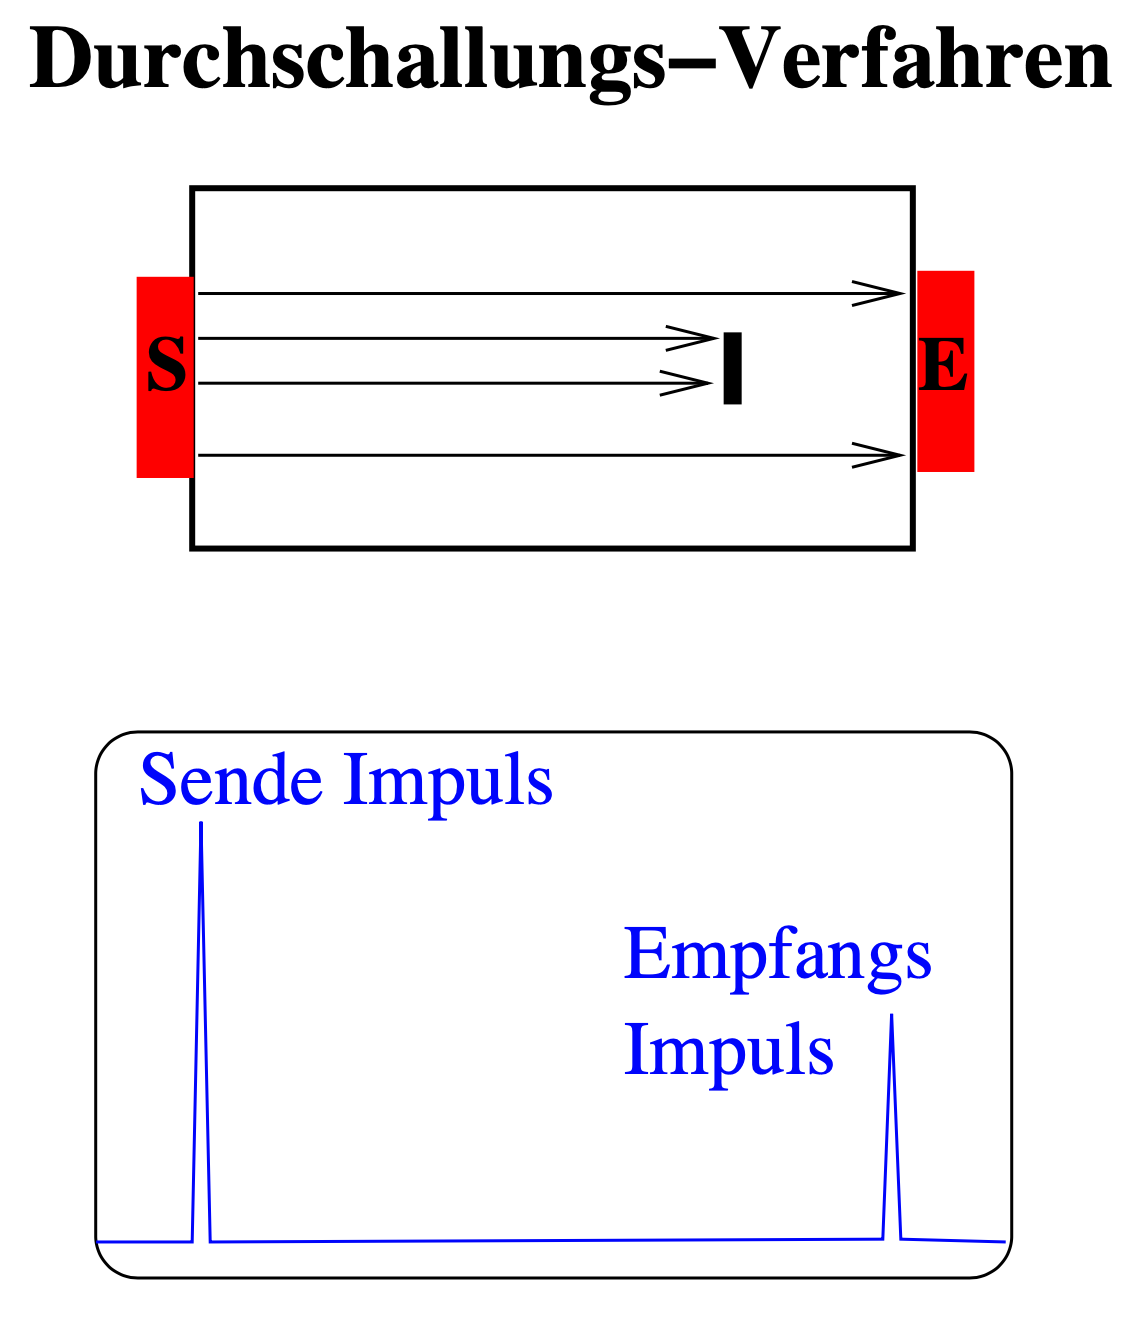
\includegraphics[width=0.4\textwidth]{bilder/Durchschallungs-Verfahren.png}
    \caption{Bild Durchschallverfahren}
\end{figure}
\subsubsection{Impuls-Echo-Verfahren}
Beim Impuls-Echo-Verfahren befinden sich Sender und Empfänger beide auf der gleichen Seite der Probe und über die Laufzeit lässt sich somit auch die Lage der Fehlstelle bestimmen.
\begin{equation}
    s = \frac{1}{2}ct \nonumber
\end{equation}
\begin{figure}[H]
    \centering
    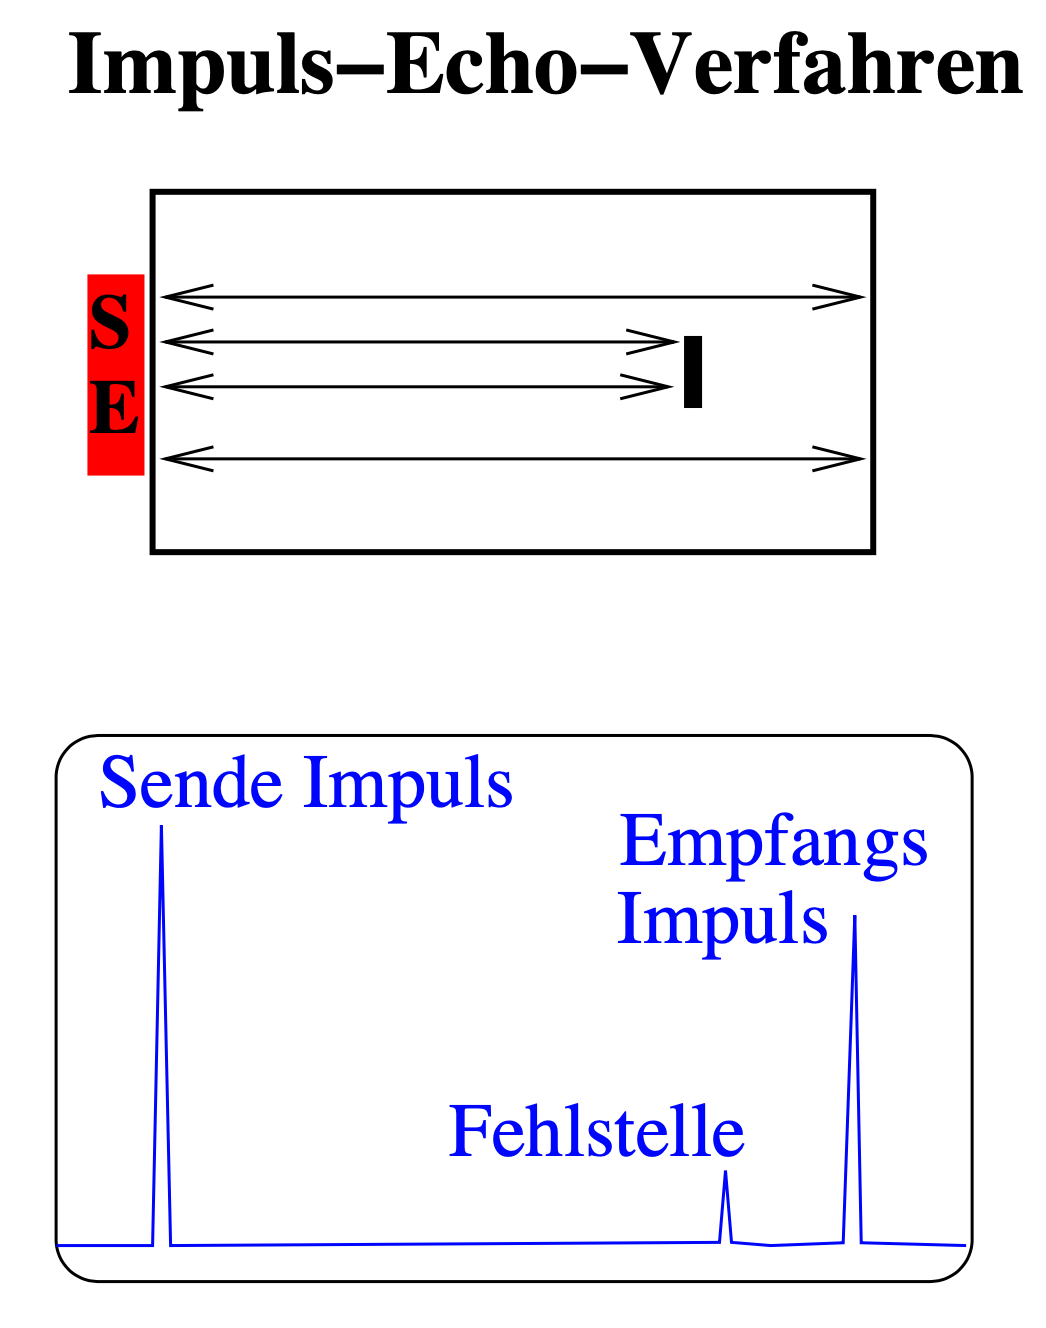
\includegraphics[width=0.4\textwidth]{bilder/Impuls-Echo-Verfahren.png}
    \caption{Bild Impuls-Echo-verfahren}
\end{figure}
